\documentclass{article}
\usepackage[UTF8]{ctex}
\usepackage{geometry}
\usepackage{multirow}
\usepackage{natbib}
\geometry{left=3.18cm,right=3.18cm,top=2.54cm,bottom=2.54cm}
\usepackage{graphicx}
\pagestyle{plain}	
\usepackage{setspace}
\usepackage{enumerate}
\usepackage{caption2}
\usepackage{datetime} %日期
\renewcommand{\today}{\number\year 年 \number\month 月 \number\day 日}
\renewcommand{\captionlabelfont}{\small}
\renewcommand{\captionfont}{\small}
\begin{document}

\begin{figure}
    \centering
    
\includegraphics[width=8cm]{upc.png}

    \label{figupc}
\end{figure}

	\begin{center}
		\quad \\
		\quad \\
		\heiti \fontsize{45}{17} \quad \quad \quad 
		\vskip 1.5cm
		\heiti \zihao{2} 《计算科学导论》个人职业规划
	\end{center}
	\vskip 2.0cm
		
	\begin{quotation}
% 	\begin{center}
		\doublespacing
		
        \zihao{4}\par\setlength\parindent{7em}
		\quad 

		学生姓名:\underline{\qquad  赵广浩 \qquad \qquad}

		学\hspace{0.61cm} 号:\underline{\qquad 2116010227\qquad}
		
		专业班级:\underline{\qquad 计科2104 \qquad  }
		
        学\hspace{0.61cm} 院:\underline{计算机科学与技术学院}
% 	\end{center}
		\vskip 1.5cm
		\centering
		\begin{table}[h]
            \centering 
            \zihao{4}
            \begin{tabular}{|c|c|c|c|c|c|c|c|c|}
            % 这里的rl 与表格对应可以看到,姓名是r,右对齐的;学号是l,左对齐的;若想居中,使用c关键字。
                \hline
                \multicolumn{5}{|c|}{分项评价} &\multicolumn{2}{c|}{整体评价}  & 总    分 & 评 阅 教 师\\
                \hline
                自我 & 环境 & 职业 & 实施 & 评估与 & 完整性 & 可行性 &\multirow{2}*{} &\multirow{2}*{}\\
                分析& 分析& 定位 & 方案 & 调整 & 20\% & 20\% & ~&~ \\\            
                10\% & 10\% & 15\% & 15\% & 10\% & &  &~ &~\\
                \cline{1-7} 
                & & & & & & & ~&~ \\
                & & & & & & & ~&~ \\
                \hline      
            \end{tabular}
        \end{table}
		\vskip 2cm
		\today
	\end{quotation}

\thispagestyle{empty}
\newpage
\setcounter{page}{1}
% 在这之前是封面,在这之后是正文
\section{自我分析}
\subsection{自然条件}
性别、年龄、身体条件、健康状况、居住城市等。\par
我性别男,年龄20周岁,身体条件良好,平时有长期保持打篮球、健身的运动习惯,身心健康状况均良好。籍贯山东德州,现居地山东青岛。\par
性别:由于性别平等的现代社会,性别对大多数职业选择的限制已经减小。然而,某些行业仍可能存在一些特定的性别倾向。\par
年龄:20岁是一个年轻有活力的阶段,可能会面临一些对于初入职场的挑战,但同时也有机会更快地适应新的工作环境。自己可以利用这个阶段积累经验,不断学习和发展自己的职业技能。\par
身体条件和健康状况:我良好的身体条件和健康状况对于职业发展是有利条件。有助于提高工作效率,增强抗压能力,对于互联网行业“码农”等工作量大或长时间工作的职业尤为重要。\par
运动习惯:对于自己打篮球和健身的习惯,一是有助于维持身体健康和提高工作效率,在工作之余可以起到放松解压的作用,二是对团队合作、人际关系交往、领导力等方面有一些优势,这在职场中也是受欢迎的特质。\par
居住城市:自己对于回乡发展的想法并不大,青岛这样的城市可能提供了更多的职业机会和社交资源,同时自己目前是升学规划,将来可能会去到不同的城市。城市的发展也可能带来不同领域的工作机会,自己可以考虑利用所在城市的资源来寻找更适合自己发展的职业。\par
\subsection{性格分析}
我性格外向,开朗乐观,喜欢交朋友,共情能力强,沟通和协调组织能力强但性格方面也存在一些缺陷:好胜心强,较为自我、不易接受他人的建议和批评,易内耗,有较为严重的拖延症。\par
团队合作:我喜欢交朋友,社交欲望强烈,在团队中表现向来较为出色。因为自己的开朗和外向,一般会成为团队氛围的积极推动者,促进合作和良好的工作关系。\par
领导潜力:自己担任组长和班长的经历较多,具备沟通和协调组织能力,这些都是领导者所需要的关键技能。你可能在领导职责中脱颖而出,能够有效地组织和激励团队成员。\par
社交网络:喜欢交朋友使我构建了一个较大的人际关系网,尤其是学长学姐们的经验对于我职业发展和信息的获取非常有帮助。\par
共情能力:具有强大的共情能力使我经常理解和关心他人的感受,这在以后的工作中建立良好的人际关系和解决问题时非常重要。\par
好胜心强:在推动自己前进的同时也会带来一些问题,可能导致一些竞争性的情境而忽视了保持合作关系的重要性。\par
较为自我:对自己的自我意识较强可能使我在某些情境下难以接受他人的观点,从而影响了团队合作和集体决策。\par
易内耗和拖延:经常会对学习和工作产生负面影响。自己应尝试建立良好的时间管理习惯,制定清晰的工作计划,以减少拖延的可能性。\par
\subsection{教育与学习经历}
\begin{table}[h]
	\centering
	\caption{教育与学习经历}
	\begin{tabular}{llc}
		% 这里的rl 与表格对应可以看到,姓名是r,右对齐的;学号是l,左对齐的;若想居中,使用c关键字。
		\hline
		时间 & 学校 & 职务\\
		\hline
		2009.9-2015.6 & 山东省德州市禹城市步云小学 & 学生 \\ 
		2015.9-2018.6 & 山东省德州市禹城市齐鲁中学 & 学生 \\
		2018.9-2021.6 & 山东省德州市禹城市第一中学 & 学生 \\
		2021.9-至今 & 中国石油大学(华东) & 学生 \\
		\hline
	\end{tabular}
	\label{table1}
\end{table}
\begin{itemize}
	
\item 2009.9-2015.6期间,我就读于山东省德州市禹城市步云小学,小学期间得益于母亲的教育,每天辅导我的功课,学习成绩经常在年级前几名。自己从小学开始就是一个好胜心很强的孩子,从不只满足于成绩,努力在各方面做好,想要成为老师和家长口中那个别人家的孩子,在学校里算是受到老师们的喜爱,一直担任班级的班长。小学期间在课余上了四年的英语辅导班,为自己之后的英语学习打下了较好的基础。同时学习了一年的书法兴趣班、一年的围棋兴趣班、两年的跆拳道兴趣班、三年的篮球兴趣班,虽然坚持到现在的只有篮球这项运动,但还是开拓了自己的视野,尤其是培养起了运动的习惯。\par
\item 2015.9-2018.6期间,我就读于山东省德州市禹城市齐鲁中学,初中期间成绩较小学有所退步,但仍稳定在年级前五十名,在班内任职三年班长。因为自己身边有着同样一群热爱数学的同学和一位极其负责且幽默风趣的数学老师,自己在初中最大的学习收获便是对数学的热爱和逻辑思维能力的提升,同时也为高中时期参与信息竞赛学习打下基础。由于综合成绩一直较好,初三上学期便通过提前批招生录取至当地第一中学竞赛班。初中学习了三年萨克斯兴趣班,通过萨克斯业余十级和音乐理论知识二级考核。\par
\item 2018.9-2021.6期间,我就读于山东省德州市禹城市第一中学,由于自己是提前批录取,在中考之前便开始了高中科目的学习,同时参与竞赛班选拔,自己第一次接触信息竞赛便深深为之吸引,还记得第一次照老师的葫芦画瓢地输出那句“hello world”时激动的心情。竞赛的这片绿茵从不缺乏天才,但我深知其实自己从来就没有什么天赋,有的只是对编程的一腔热爱和努力,从此无论是自习还是体育课,有空闲时间的机会我便会到学校机房学习算法。2018年11月,在入学半年后,通过选拔在队内11人中脱颖而出,成为高一唯一一名参与noip的队员并获山东省二等奖。2019年再次获得二等奖后退出竞赛队伍转战高考。\par
\item 2021.9-至今,我就读于中国石油大学(华东)测绘工程专业,高考失利但得益于自己的竞赛经历,通过综合评价提前批录取至我校测绘工程专业就读。在进入专业的学习之后发现测绘工程的学习和工作并不适合自己,在了解学校相应转专业政策后,大一上学期努力学习,在大一下学期以测绘工程专业第一名的成绩转入计算机科学与技术专业,并当选计科2104班班长,自转入至今专业排名稳定在前10\%。 
\end{itemize}
\subsection{工作与社会阅历}
\begin{itemize}
	
\item 政治面貌:中共党员,作为计算机科学与技术学院21级第一批中共党员,我时刻保持党员的标准和要求,勇于担当为人民服务。大一期间在学院党建中心参与工作,提高自己的党性修养,目前担任计科2304班驻班党代表,发挥自己的模范带头作用,暑假期间牺牲自己休息时间为学弟学妹开展入学教育班会、对培养方案进行答疑解惑、开学后开展游园会等。\par
\item 学生工作:小学六年担任班级班长,初中三年担任班级班长,高中三年担任班级班长,大学期间大一担任院学生会干部,作为主要负责人组织策划了院校级文体活动十余项、累计受众前余人,大二期间担任班级班长,班级连续两个学期达到优良学风班标准,及格率达到100\%。\par
\item 社会实践与志愿服务:曾多次参与家乡的社区志愿服务活动,管理公益图书馆管理,无偿为社区学生上课、作业辅导等;还曾参与回母校宣讲社会实践,向母校百余名学弟学妹在科研实力等方面介绍石大风采;疫情期间我积极参与学校志愿服务,累计服务市场50余小时。\par
 
\end{itemize}
\par 这些丰富的工作与社会阅历对我的职业规划产生了积极的影响。首先,党员身份和党性修养使我在职业生涯中更注重服务人民、履行社会责任。其次,学生工作经历培养了我的领导力、组织协调能力,为未来从事管理与领导工作打下坚实基础。社会实践和志愿服务则锻炼了我的人际交往和沟通能力,使我更具社会责任感。综合而言,这些经历不仅增强了我的综合素质,也为我未来的职业规划提供了丰富的资源和经验。
\subsection{知识、技能与经验}
\begin{itemize}
	
\item 基础知识:数学、物理、化学、生物等理科基础扎实\par
\item 英语能力:CET-4:527分 CET-6:526分,均为一次性通过成绩\par
\item 专业能力:高中时期学习信息学竞赛,拥有一定的算法能力;大学期间专业课成绩较好,程序设计100分,数据结构、数字逻辑电路、大学计算机等专业课程95分以上,十余门课程成绩90分以上\par
\item 技能:具备良好的编程习惯和较强的分析能力,熟悉C/C++、Python、Java等编程语言,熟悉mysql的语句以及使用,掌握html、php、xml等语言,具备一定的软件开发能力;大二暑假自学软件测试,掌握测试用例的编写和使用postman进行抓包,熟练掌握功能测试方法,了解并会使用部分pytest框架进行自动化测试,具备一定的软件测试能力;大三主动联系导师进组,目前熟悉markdown、latex语法,掌握visio、draw.io等作图软件的使用,有较多的科研论文阅读经历,具备一定的科研经验。\par
 
\end{itemize}
\par 综合来看,我的知识与技能较为多方面,但还都只是浅尝辄止不够精进,但同时也使得我在算法、测试开发等技术岗位和科研等领域都有广泛的选择。我可以根据自己后期的个人兴趣和职业目标,选择一个更符合自己发展方向的职业,不论是技术型岗位还是更注重管理、研发的方向。
\subsection{兴趣爱好与特长}
\begin{itemize}
	
\item  爱好运动并长期保有运动习惯,对于篮球,七年以来保持了至少一周一打的频率;喜欢健身,至少一周三练的健身频率已保持半年;偶尔长跑,中考一千米3:28夺得满分,大学体测一千米3:23打破个人记录。\par
\item  音乐方面个人爱好是吹萨克斯,虽大学期间有所怠慢,但仍保持强烈的肌肉记忆和热爱。\par
\item  喜欢看各种文学作品,尤其是小说电影等,对科幻、悬疑题材较为感兴趣,但没有形成定期阅读的习惯。\par

\end{itemize}
\par 篮球和健身锻炼培养了我的团队协作和领导力,这对于职场中与团队协作、领导项目的能力提升有帮助。可以在团队合作密切的行业或公司寻找机会,考虑与其他团队成员协同工作的职位。长期坚持运动也表明我有一定的自律能力,这对于面对挑战和完成工作任务时的耐心和毅力是有益的。我也可以在需要耐心和自律的职业领域寻找机会,如项目管理、研发等。\par
掌握萨克斯的才艺展示可以使得我在公司或学校的文化活动中担任一些角色,对文学作品的热爱可能使得我在工作之余与同时之间拥有更多的交流话题,有利于维持人际关系。
\section{环境分析}
\subsection{社会环境分析}
\begin{itemize}
	
\item 政治形势:\par
中国目前的政治形势呈现出一种社会主义制度的稳定局面,由中共中央领导的政治体制主导整个国家。近年来,中国政府提出并实施了一系列政策和改革措施,旨在推动国家的经济、社会和文化发展。新发展理念、全面深化改革、依法治国等理念成为国家治理的核心。中国政治体系强调党的领导地位,通过建设中国特色社会主义事业来实现国家现代化的宏伟目标。同时,中国积极参与国际事务,推动全球治理体系的改革,提出了一系列国际合作倡议,如“一带一路”等,展示了对于全球事务的积极参与和引领。总体而言,中国当前的政治形势在维持政治稳定的同时,不断进行着制度性和政策性的调整,以适应国内外环境的变化,致力于实现国家富强、人民幸福的目标。\par
\item 经济形势:
\begin{enumerate}
	\item 经济发展进入了高质量发展阶段,强调提升增长的质量和效益。政府推动供给侧结构性改革,注重技术创新和科技进步。新经济领域如数字经济、人工智能、大数据等蓬勃发展,成为经济增长的新引擎。
	\item 消费升级,随着居民收入水平提高,消费结构逐渐升级,服务业和高端消费逐渐崭露头角。同时,中国经济逐渐从出口和投资驱动向消费驱动转变,表现出更为平衡和可持续的趋势。
	\item 绿色发展成为国家发展的重要方向,政府出台了一系列环保政策,鼓励清洁能源和绿色技术的应用,以及低碳发展。此外,中国积极参与全球经济合作,推动“一带一路”倡议,加强与其他国家的贸易、投资和科技合作,展示出开放合作的姿态。
	\item 金融领域也在经历改革,以提高金融服务实体经济的效率。资本市场改革、降低企业融资成本等政策都在推动着金融体系的调整和创新。
	\item 当前经济运行面临新的困难挑战,主要是国内需求不足,一些企业经营困难,重点领域风险隐患较多,外部环境复杂严峻。疫情防控平稳转段后,经济恢复是一个波浪式发展、曲折式前进的过程。
\end{enumerate}
\item 就业形势:\par
\par 大学生就业形势在当前社会背景下面临着一系列挑战和机遇。随着高等教育的普及,大学毕业生规模逐年扩大,使得就业市场更加竞争激烈。同时由于疫情等因素,一些传统行业和中小微企业受到较大冲击,导致一些毕业生在求职过程中面临更大的竞争和不确定性,例如目前很多企业出现了校招名额缩减甚至取消春招的现象,许多大厂更是不断裁人。\par
\par 今年考研人数减少36万,考公人数增加41万人,我认为更是从一定程度上说明了学历贬值的问题,同时找工作难,大家更期望体制内的稳定工作。
\end{itemize}
\subsection{家庭环境分析}
\begin{itemize}
	
\item 婚姻状况:未婚。\par
\item 经济状况:目前经济来源主要来自父母每月提供的生活费,奖学金、勤工俭学占少部分经济来源。\par
\item 家人期望:家人期望我继续攻读硕士研究生,研究生毕业后,选调或是考公至山东济南或者青岛并定居,定居工作稳定后考虑在本地结婚生子。\par
\item 家人传统:父母以及各长辈大部分为体制内工作者,不希望自己进入企业内工作。
 
\end{itemize}
\subsection{职业环境分析}
\begin{itemize}
\item 行业现状及发展趋势:《中国互联网企业综合实力指数》表明2022年我国互联网综合实力企业呈现如下特征:\par
\begin{figure}[h!]
	\centering
	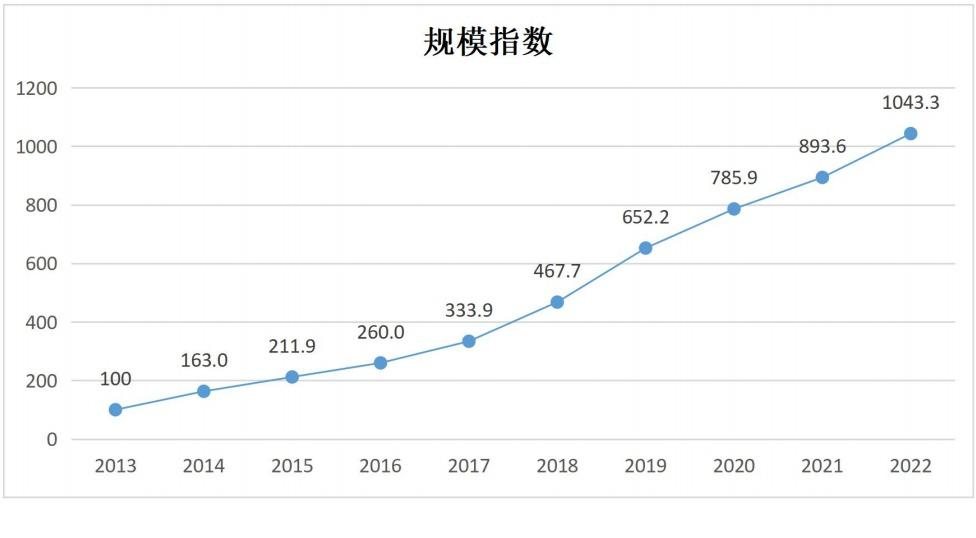
\includegraphics[width=8cm]{guimo}
	\caption{中国互联网企业综合实力指数——规模指数}
	\label{fig:guimp}
\end{figure}
一是近十年来,互联网企业综合实力逐年增强,行业呈持续发展态势;二是营业收入和营业利润均呈上升态势;三是研发投入持续加码,发明专利数量呈增长态势。四是产业互联网持续发展;五是风险防控能力处于健康水平;六是互联网企业纳税总额稳步提升等。\par
从招聘需求角度来看,猎聘大数据研究院发布《2022年紧缺人才薪酬报告》如下:\par
\begin{figure}[h!]
	\centering
	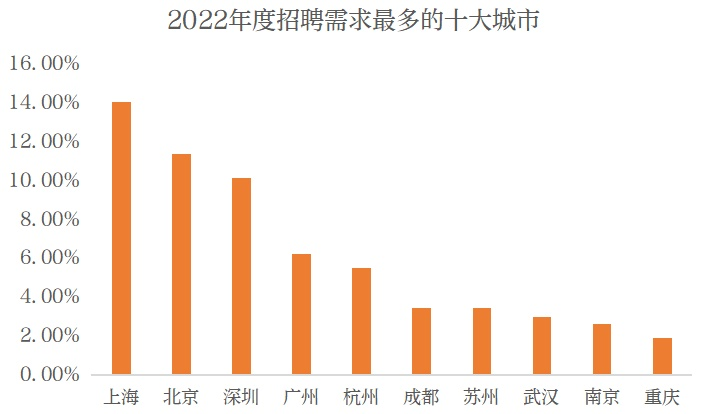
\includegraphics[width=8cm]{zhaopin}
	\caption{2022年度招聘需求最多的十大行业}
	\label{fig:zhaopin}
\end{figure}
数据显示,从行业需求来看,2022年度招聘需求最多的行业就是IT互联网。在招聘平均年薪方面,金融、IT/互联网/游戏、电子/通信/半导体位居行业前三,分别为26.59万、26.21万、25.84万元。\par
互联网方面,架构师、算法工程师、Golang程序员等紧缺岗位年度薪酬最高,均值皆达50万元以上,新媒体运营岗位年度薪酬相对最低,均值仅为18.85万元。据国家统计局数据显示,2021年信息传输、软件和信息技术服务业年平均工资为20.15万元,同比增速13.5。\par
\begin{figure}[h!]
	\centering
	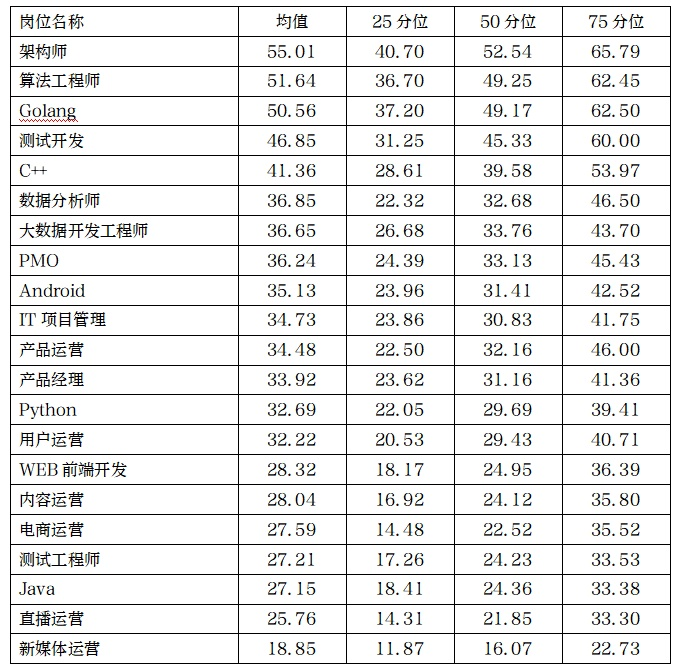
\includegraphics[width=8cm]{xinchou}
	\caption{2022年岗位及平均薪酬}
	\label{fig:xinchou}
\end{figure}
\item 互联网职业的工作内容与工作要求:\par
\begin{enumerate}
\item 技术类\par
管理职位:CTO、技术合伙人、技术经理、技术总监、运维总监、测试总监、架构师、项目总监、安全专家、科学家等\par
基础职位:后端开发、前端开发、人工智能、测试、运维、数据库管理、硬件开发、企业软件

\item 产品类\par
管理职位:产品总监、游戏制作人、设计总监、设计主管、用户研究总监等\par
基础职位:产品经理、产品设计师、用户研究\par

\item 运营类\par
管理职位:主编、运营总监、COO、客服总监等\par
基础职位:运营、编辑、客服\par

\item 市场类\par
管理职位:策划经理、媒介经理、市场总监、公关总监、创意总监、渠道总监等\par
基础职位:市场营销、媒介公关、品牌/广告、渠道推广等\par

\item 销售类\par
管理职位:销售总监、商务总监、区域总监、城市总监、团队经理等\par
基础职位:销售专员\par

\item 职能类\par
管理职位:行政总监、财务总监、HRD等\par
基础职位:人力资源、行政、财务、法务等\par

\item 设计类\par
管理职位:设计经理/主管、设计总监、视觉设计经理/主管、视觉设计总监、交互设计经理/主管、交互设计总监、用户研究经理/主管、用户研究总监\par
基础职位:视觉设计、交互设计\par
\end{enumerate}
\item 互联网职业的发展前景:尽管互联网行业发展迅猛,但也要注意一些挑战,如激烈的竞争、技术更新换代快、安全和隐私问题等。因此,互联网从业者需要保持学习和适应能力,不断提升自己的技能水平,以保持在这个变化迅速的行业中的竞争力。总体来说,互联网职业在未来仍将是一个充满机遇的领域。

\end{itemize}

\subsection{地域与人际环境分析}
\begin{itemize}
\item 济南的气候水土、文化特点、发展前景:\par
山东济南地处温带季风气候区,夏季相对温暖,冬季相对寒冷。四季分明,春季温暖宜人,夏季相对炎热,秋季凉爽宜人,冬季寒冷干燥。济南地势较为平坦,以泉水众多而著称,拥有历史悠久的“72名泉”之一——趵突泉。农业方面,山东是中国的粮食生产大省,水土资源丰富,有助于农业和园林业的发展。\par

\begin{figure}[h!]
	\centering
	
\includegraphics[width=8cm]{baotuquan}
	\caption{济南趵突泉}
	\label{fig:baotuquan}
\end{figure}

济南作为历史文化名城,拥有丰富的历史文化遗产,如千佛山、大明湖等,各类历史古迹和博物馆丰富着城市文化内涵。山东是齐文化的发源地之一,具有深厚的文学艺术传统,齐鲁书院是古代文学艺术的重要殿堂。山东以鲁菜著称,济南作为山东省省会,承载着浓厚的鲁菜文化,有着独特的饮食传统。
\begin{figure}[h!]
	\centering
	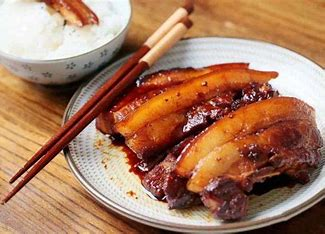
\includegraphics[width=8cm]{lucai}
	\caption{济南把子肉}
	\label{fig:lucai}
\end{figure}

作为山东省省会,济南一直是经济的重要节点,未来可望继续成为先进制造业和现代服务业的重要基地,推动经济的可持续增长。政府在科技创新上投入不断增加,济南正逐渐崭露头角成为科技创新的重要城市,特别是在新一代信息技术、生物科技等领域。

\item 济南的人脉与人际关系:
\par 因为自己的家庭是地地道道的山东家庭,位居山东德州距离济南一两个小时车程,所以自己家的很多亲戚都在济南定居,比如在济南中石油工作的表哥等等,自己家庭在济南的人际关系都会对自己的职业发展起到优势作用。

\item 青岛的气候水土、文化特点、发展前景:\par
\par 青岛地处亚热带季风气候区,四季分明,夏季相对凉爽,冬季相对温和。由于临海的地理位置,青岛气候湿润,降水相对充沛。地势较为平坦,土壤质地较好,适宜农业发展。青岛的海岸线曲折,拥有许多美丽的海滩和自然景观,是一个宜居城市。

\par 青岛是一座海洋城市,深受海洋文化影响。这体现在建筑风格上,如德国建筑风格的典范——栈桥,以及在饮食文化中,以海鲜为主的独特口味。由于历史原因,保留了大量的德国建筑,城市风貌融合了中西文化元素,呈现出一种独特的欧洲风情。 青岛啤酒是中国最著名的啤酒品牌之一,青岛啤酒节等活动常年举办,体现了浓厚的啤酒文化。青岛是文艺气息浓厚的城市,有许多文艺活动、艺术展览和文学创作,吸引着文艺青年和艺术家。
\begin{figure}[h!]
	\centering
	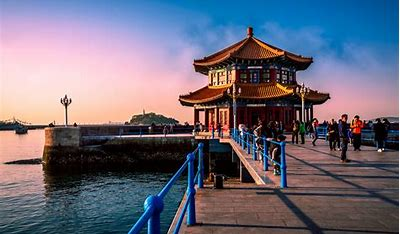
\includegraphics[width=8cm]{zhanqiao}
	\caption{青岛栈桥}
	\label{fig:zhanqiao}
\end{figure}

青岛是中国重要的沿海城市,经济实力较强。作为山东省的经济引擎,青岛未来将继续推动现代服务业和高技术产业的发展,提升经济水平。青岛积极推动科技创新,特别是在海洋科技、生物医药等领域,未来将成为国家科技创新的重要基地。 青岛具有独特的城市风光和海滨景观,旅游业一直是支柱产业。未来随着国内外游客需求的增加,青岛的旅游业有望进一步繁荣。

\item 青岛的人脉与人际关系:
\par 因为自己本科在中国石油大学(华东),认识了很多定居在青岛的老师,和很多留青发展的学长学姐,学校的资源和人脉也会为自己的职业发展有益。
\end{itemize}
\begin{figure}[h!]
	\centering
	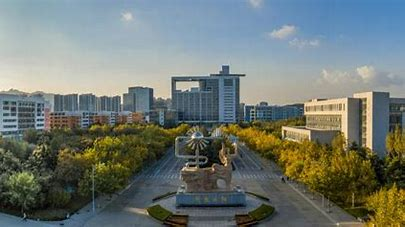
\includegraphics[width=8cm]{upcc}
	\caption{中国石油大学(华东)}
	\label{fig:upcc}
\end{figure}

\par 

\section{职业定位}

\subsection{行业领域定位与理由}
自己将会从事计算机行业,理由如下\par
\begin{enumerate}
	\item 兴趣和热爱:我在小学时期的微机课上第一次接触计算机,在高中时期学习信息学算法竞赛,大学义无反顾转专业至计算机科学与技术,可以说计算机已经成为了贯穿我人生始终的伙伴。我永远忘不掉自己第一次输出“hello world”时欣喜的感觉,忘不掉自己做不出算法题疯狂怀疑自己的智商,忘不掉为了学好专业课在南教通宵的日日夜夜。我享受并一直热爱着,我希望他成为我的工作,继续书写我们的故事,这种热爱和兴趣将成为我在工作中持之以恒努力的动力。
	\item 高薪和就业机会:计算机行业有较高的薪资水平,同时该领域一直是市场需求旺盛的行业之一。计算机专业的就业机会较为广泛,既可以选择进入私企、大厂,也可以考取公务员编制。计算机行业就业的灵活性符合我的职业规划,提供了多样的职业选择。。
	\item 办公条件优越:相对于测绘工程等需要在户外或者特殊环境下工作的行业,计算机行业的办公环境通常更为舒适和优越。这对于长期从事这个行业的人来说,是一个额外的福利。
\end{enumerate}
\subsection{职业岗位起点定位与理由}
自己可能优先会进入一家济南或者青岛的国央企从事软件开发或测试的岗位,后期考虑转型至管理岗;也有可能会考取选调生。\par
\begin{enumerate}
	\item 选择国央企的原因是基本符合自己对目标工作钱多事少的要求,虽然自己想从事计算机行业,但是并不喜欢996的工作节奏,而国央企相对于私企更为稳定轻松,通常有着较为轻松的工作氛围,符合我对工作生活平衡的追求;同时相对于公务员事业编薪资更高;且自己目前有升学至985院校的规划,而国有企业较多对学历有一定要求,这与我的未来规划较为契合。
	\item 从事软件开发或测试岗的原因是自己对测试开发的内容掌握较为熟悉,且随着信息技术的不断发展,软件开发和测试等相关岗位的需求一直保持相对较高水平。选择这个岗位有望在职业生涯中享有较好的就业前景。又因为在软件开发或测试中,通常需要与团队成员协作,共同解决问题,完成项目,有助于发挥自己团队协作和沟通能力的优势,提高工作效率。
	\item 与直接考取公务员相比,选调生的难度相对较低,更符合我目前的实际情况。我作为中共党员,同时在学生工作方面有着丰富的经历,在选调生的选拔中可能会起到一定的优势作用。
\end{enumerate}
\subsection{职业目标与可行性分析}
\par
\begin{enumerate}[(1)]
	\item 短期目标(大学4年)
	\begin{itemize}
		\item 成果目标:明年成功拿到研究生推免名额并报送至一所中流985院校攻读计算机专硕,大四在青岛找一家公司进行测开岗位的实习。
		\item 经济目标:大学期间拿一次国家奖学金,补贴家用。
		\item 能力目标:提升自己的科研能力,争取明年在组内发表一篇一作CCF-C类会议。
		\item 职务目标:继续担任班级班长的工作,提升自己的工作能力。
	\end{itemize}
	\item 中长期目标(5-10年)。
	\begin{itemize}
		\item 成果目标:研究生期间好好科研好好生活,顺利毕业后进入一家国央企工作,工作定居后如果有合适人选考虑结婚。
		\item 经济目标:研究生期间不向家里要钱,实现完全经济独立。第一年工资薪酬达到10w+。
		\item 能力目标:研究生期间顺利发表论文,研二时尽量达到毕业目标,提前实习提升自己的工作能力,争取具备转正能力。
		\item 职务目标:工作后先从技术岗做起,工作5-10年后考虑转型至管理岗。
	\end{itemize}
\end{enumerate}

\section{实施方案}
\begin{enumerate}[1、]
	\item 如何利用现有条件和自身优势以实现职业生涯目标。\par
	\begin{itemize}
		\item 短期目标方案:保持好自己专业前10\%的成绩,加上自己B类国一的奖项,推免名额应该是可以拿到,接下来努力科研积极参加竞赛,争取发表一作论文并拿到一项A类国一奖项,完成保到中九的短期目标。
		\item 长期目标方案:利用大四没课在公司的实习机会,将理论知识转化为实际项目经验。通过参与公司项目,了解实际工业界需求,锻炼解决问题的能力,积累实践经验。在读研期间,有机会接触到来自各地的优秀学者和同学。利用这一优势,主动参与学术活动,拓展专业人脉。与导师和同学建立深厚的关系,将来可能成为合作伙伴或推荐人。
	\end{itemize}
	\item 如何克服缺点、弥补不足、增长知识、提高能力以实现职业生涯目标。\par
	自己目前最大的缺点就是拖延,无论是考试作业还是组会,不到ddl提不起效率。自己会将时间合理规划,尽量做到劳逸结合而不是放松的时候完全放松,忙的时候就忙到通宵。此外,我也会深入分析导致拖延的原因,主动寻找解决办法。可能是因为对任务的难度或复杂性感到压力,或者是缺乏对任务的充分理解。
	最终,我深知改变习惯需要时间和毅力,但我愿意付出努力来逐步改善自己。
	\item 如何处理人际关系和发展人脉以实现职业生涯目标。\par
	同学之间的人际关系照常保持,下一步主要是发展和学校老师之间的关系。措施就是对于任课老师,积极思考多提问题,尽量给老师留下印象,同时在参加比赛时,可以寻找较为熟悉的老师作指导教师,多和老师们沟通交流,帮老师们做一些自己力所能及的事情。
	\item 如何处理工作与家庭、生活的关系以实现职业生涯目标。\par
	秉持“工作是工作,生活是生活”的原则,绝不将工作中的脾气带到家庭和生活中来,工作没了可以再找,家庭却是我永远的后盾。工作与生活的平衡不是一场权衡取舍的博弈,而是一种和谐的状态,要以平和的心态处理工作和生活的关系。
	\item 如何处理释放工作压力、保证身心健康以实现职业生涯目标。\par
	保持自己的运动习惯,每天晚上健身撸铁,既可以保持了良好的身体状况,又成为了我释放一天压力和紧张情绪的出口。周末约朋友打打球吃吃饭,和朋友在一起的社交氛围总是轻松愉快的,大家之间也可以互相吐槽吐槽不顺利的事,也可以提出自己作为朋友不同的看法和见解。
\end{enumerate}
\par 
\section{评估与调整}
\subsection{评估时间}
每学期评估一次。\par
\subsection{评估内容}
\begin{itemize}

\item 成果目标:关注大三下学期的成绩排名,确保成绩保持在了专业前10\%以达到部分学校预推免的要求,同时关注竞赛最高奖项有没有拿到A类国一。若成绩下滑,则大三下学期抓紧稳住排名,不能掉出前10\%。若竞赛未拿到国一,则重新评估竞赛加分情况,并考虑是否完全调整重心至科研方面。\par
\item 经济目标:根据自己上学期的成绩评估是否能拿到国家奖学金,如果无法获得,将认真考虑大四实习的问题,寻找适当的机会提高经济收入。\par
\item 能力目标:专注于研究论文,确保自己已经具备成熟、可行和创新的idea。如果论文进展不如预期,我将主动与导师交流,确保此段科研经历能够为未来的参营活动提供有力的支持。\par
\item 职务目标:考虑到保研的情况,在大四时评估是否重新担任班长职务。如果保研成功,将继续考虑并决定是否继续承担班长职责,为自己和同学们创造更好的学习环境。\par
	 
\end{itemize}
\subsection{调整原则}
灵活性与适应性:在追求目标的过程中,保持灵活性,及时根据实际情况做出调整。学业和竞赛可能受到各种因素的影响,因此需要在计划中加入一些弹性,以适应变化。

优先级与时间管理: 给每个目标设定清晰的优先级,并合理分配时间。考虑到保研的重要性,可以将学业和竞赛的时间分配在保研准备之外,确保在关键时刻有足够的精力和时间投入。

实时监控和反馈:设定目标后,定期进行监控和反馈,检查进展情况。如果发现某个目标的实现存在问题,及时调整计划,采取有效的措施,以确保整体目标的达成。

资源的有效利用: 确保在追求目标的过程中,充分利用现有资源,包括学校提供的各种学科和实践机会,导师的推荐机会,学长们的保研面经,以及计算机保研群中的资源。

自我关怀和平衡: 在追求目标的同时,注意保持身心健康。合理安排休息时间,保证充足的睡眠,有助于提高学习和工作效率,过度压力可能会对目标的实现产生负面影响。

沟通与反馈: 与导师、同学、朋友等建立有效的沟通机制。分享目标,获取他们的意见和建议,从中获得更全面的支持和反馈,有助于更好地调整计划。

自我激励与奖励: 设立一些小的、可量化的里程碑目标,并为实现这些目标设立奖励机制。这有助于保持积极性,提高工作和学业的动力。
\section{报告仓库地址}
https://github.com/zgghh/Course\_Introduction-to-Computational-Science
\end{document}
